\chapter{Analisador Estático e Caracterização do Uso de Construções da Linguagem Java}\label{cap:arquiteruta}

Com o intuito de obter uma compreensão sobre o uso das construções da linguagem Java, tornou-se necessária a implementação de uma ferramenta de análise estática de propósito específico, por outro lado com capacidade de ser extensível para extrair diferentes tipos de informações. Utilizando esse suporte ferramental, descrito na Seção \ref{sec:ferramenta}, foi conduzido um estudo empírico para caracterizar o uso de construções da linguagem Java, cujos resultados 
estão descritos na Seção \ref{sec:resultados}.

Um ponto de extrema relevância na construção do \NOMESOFTWARE é que este deveria ser de fácil manipulação para desenvolvedores com pouca experiência no domínio desta aplicação. Com isso respeitando os padrões adotados neste trabalho que serão detalhados nas subseções \ref{subsec:entradaAS}, \ref{subsec:classeModelos} e \ref{subsec:criacaoVisitors} qualquer programador pode criar \textit{Visitors} para pesquisar por construções de suas necessidades.

\section{Visão Geral do \NOMESOFTWARE}\label{sec:ferramenta}

A Figura~\ref{fig:Arquitetura} apresenta uma visão geral dos elementos que compõem o analisador estático desenvolvido durante a condução deste trabalho de graduação. Em linhas gerais, tal suporte ferramental recupera do sistema de arquivos todos os arquivos contendo código fonte escrito na linguagem Java, realiza o \textit{parse} desses arquivos gerando uma representação intermediária correspondente, mais adequada para as análises de interesse deste projeto, aplica uma série de mecanismos de análise estática  para coletar as informações sobre o uso das características da linguagem de programação e, por fim, gera os resultados no formato apropriado para as análises estatísticas no contexto deste projeto, foi feita a opção pelo formato \acs{CSV}.

Atualmente existem diversas ferramentas e bibliotecas de programação que auxiliam a construção de analisadores estáticos,  
conforme as nossas necessidades.Entretanto, devido a maior experiência dos participantes do projeto com uso da linguagem Java, foi feita a opção por se utilizar a infraestrutura da plataforma \textit{Eclipse Java Development Tools}~\cite{EclipseJDT} (Eclipse JDT). O Eclipse JDT fornece um conjunto de ferramentas que auxiliam na construção 
de ferramentas que permitem processar código fonte escrito na linguagem de programação Java. A plataforma Eclipse JDT é composta por 4 componentes principais: APT, \textit{Core}, \textit{Debug} e UI~\cite{EclipseJDT}. Neste projeto a plataforma foi usada essencialmente através do \textit{JDT Core}, que dispõe de uma representação Java para a navegação 
e manipulação dos elementos de uma árvore sintática \acs{AST} gerada a partir do código fonte, onde os elementos 
da representação correspondem às construções sintáticas da linguagem (como pacotes, classes, interfaces métodos e atributos). 

A \acs{AST} provida pelo \acs{JDT} que é composta por 122 classes, como, por exemplo, existem 22 classe para representar sentenças  como \textit{IF-Then-Else, Switch, While, BreakStatement} entre outras. Existem cinco classes que trabalham exclusivamente com métodos referenciados e seis classes exclusivas que tratam os tipos declarados, como classes, interfaces e enumerações em Java. O Eclipse JDT \cite{EclipseJDT} disponibiliza ainda um \textit{parser} 
para a linguagem Java que atende a especificação Java 8 da linguagem e que produz a representação intermediária baseada no conjunto de classes Java mencionado anteriormente e que corresponde a uma~\acs{AST} do código fonte. A plataforma também oferece uma hierarquia de classes para travessia na \acs{AST}, de acordo com o padrão de projeto \textit{Visitor} \cite{Gamma:1995}, e que facilita a análise estática de código fonte.

O padrão de projeto \textit{Visitor}~\cite{Gamma:1995} é um padrão de projeto de característica comportamental que representa uma operação a ser realizada sobre elementos de uma árvore de objetos. Neste caso, a operação a ser realizadas é visitar nós de interesse da \acs{AST} Java (como os nós que representam o uso de uma expressão Lambda em Java). 
Cada \textit{visitor} permite que uma nova operação seja criada sem que a estrutura da árvore de objetos sofra alterações, de modo que tornou-se relativamente  simples adicionar novas funcionalidades em um \textit{visitor} existente ou criar um novo \textit{visitor}.Por outro lado, a biblioteca Eclipse JDT não fornece mecanismos para 
extração e exportação de dados. Entretanto, no contexto deste projeto, foi implementado um conjunto de classes 
que visam obter maior facilidade e flexibilidade na exportação das informações coletadas durante a travessia nos nós das 
ASTs. Essa flexibilidade foi alcançada com a utilização de introspecção de código, que em Java é conhecido como \textit{reflection}. As próximas seções 3.1.1, 3.1.2 e 3.1.3 apresentam mais detalhes sobre a arquitetura e 
implementação do analisador estático, descrevendo as principais decisões de projeto relacionadas às cinco 
fases do analisador estático. 

\begin{figure}[tb]
	\center
	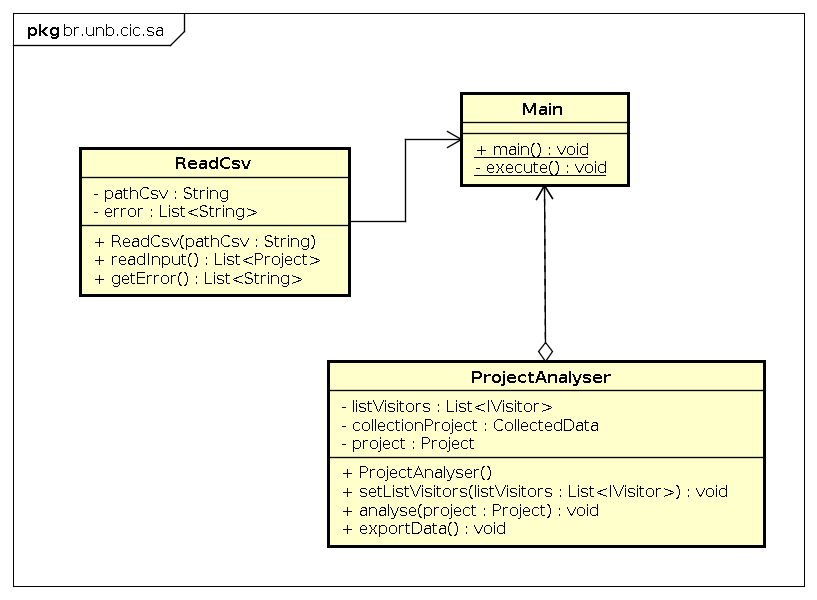
\includegraphics[scale=0.55]{Imagens/Arquitetura}
	\label{fig:Arquitetura}
	\caption{Visão geral da arquitetura do analisador estático}
\end{figure}



\subsection{Entrada do Analisador Estático}\label{subsec:entradaAS}

O analisador estático recebe como entrada um arquivo \acs{CSV} (\emph{comma-separated values}) 
que contém informações sobre os projetos a serem analisados, como nome do projeto, caminho absoluto para uma pasta no sistema de arquivos contendo o código fonte do projeto e a quantidade de linhas de código previamente computadas (conforme ilustrado na Figura~\ref{fig:Arquitetura}). 
A entrada deve ser rigidamente construído no seguindo o formato abaixo, indispensável para análise é o caminho absoluto do projeto e o nome entretanto caso não possua os outros dados deve ser mantido em branco para evitar erro no analisador.


Entrada Completa:\\
\begin{small}
\texttt{Tipo Aplicação; Inicio do projeto Ante ou Após Java 5; Nome Projeto; Versão;Caminho absoluto;Linha de código;}
\end{small}	

Entrada Incompleta:\\
\begin{small}
\texttt{;; Nome Projeto; Versão;Caminho absoluto;0;}
\end{small}


Perceba que na omissão de alguns campos estes permanecem em branco com exceção do número de linhas de código que caso seja irrelevante para análise é mantido algum inteiro, neste caso 0. Destaca-se ainda que em um único arquivo \acs{CSV} de entrada pode conter inúmeros projetos para que sejam analisados.

As informações contidas no arquivo \acs{CSV} são processadas por um conjunto de classes utilitárias que as extraem. Com o caminho absoluto informado corretamente é realizado uma verredura nesse diretório para selecionar todos os arquivos fonte da linguagem Java. Estes arquivos fonte Java são a entrada  descrita na representação abstrata do analisador estático como descrito na Figura~\ref{fig:Arquitetura}. Ou seja, para cada projeto são recuperados os arquivos contendo código fonte Java, que são convertidos para uma representação intermediária (por meio de um parser existente); processados e analisados com uma infraestrutura de \emph{visitors}, e os resultados das análises são, por fim, exportados.


\subsection{Classes Modelos}\label{subsec:classeModelos}
Após a correta elaboração da entrada descrita na subseção \ref{subsec:entradaAS} é hora de criar as classes modelos estas classes são responsáveis por mapear as informações que serão extraídas durante a fase de análise da representação intermediária. Estas classes são simples, compostas basicamente por \textit{getters - setters}. Destaca-se ainda que os métodos \textit{getters} deve conter o nome seguindo um padrão que é : \texttt{getNomeMétodo} para que o dado armazenado possar ser recuperado corretamente no fase de extração.

Como exemplo a Figura~\ref{lst:lambdaModel} exibe a simplicidade desta classe. Observe que todos os métodos \textit{getters} sem exceção deve iniciam com \texttt{get} para evitar que as informações mapeadas seja perdidas e estas classes deve ser empacote em \texttt{br.unb.cic.sa.model}.

Após a elaboração da classe modelo é necessário editar o arquivo \texttt{Beans.xml} que é um arquivo do \textit{Framework Spring} que utiliza o padrão de injeção de dependência para proporcionar um fraco acoplamento entre módulos. Este arquivo encontra-se localizado no diretório \texttt{src/main/resouces}. Para adicionar o cabeçalho correspondente do arquivo \acs{CSV} de saída que mapeará as características pesquisadas. No exemplo da Figura~\ref{lst:lambdaModel} expressão lambda que é mapeada.

Observe a forma correta de declarar este cabeçalho na Figura~\ref{lst:cabecalhoBeans}, tal declaração conterá o diretório de saída para o arquivo \acs{CSV} com as análises, o nome deste e o cabeçalho deste arquivo para facilitar o entendimento em um programa de análise como R. Posteriormente os dado mapeados neste arquivo \texttt{XML} serão referenciados na declaração dos \texttt{visitors} que também serão declarados neste mesmo arquivo a subseção \ref{subsec:criacaoVisitors} explicará detalhadamente a correata forma de criá-los.

\begin{figure}[ht]
\begin{lstlisting}[numbers=left,   numberstyle=\tiny]
package br.unb.cic.sa.model;

public class LambdaExp {

	private String file;
	private int startLine;
	private int endLine;
	private String parentMethodInvocation;
	
	public LambdaExp(String file, int startLine, int endLine){
		this.file = file;
		this.startLine = startLine;
		this.endLine = endLine;
	}

	public String getFile() {return file;}
	public int getStartLine() {return startLine;}
	public int getEndLine() {return endLine;}
	public String getParentMethodInvocation() {return parentMethodInvocation;}
			
	public void setFile(String file) {this.file = file;}	
	public void setEndLine(int endLine) {this.endLine = endLine;}
	public void setStartLine(int startLine) {this.startLine = startLine;}
	
	public void setParentMethodInvocation(String parentMethodInvocation) {
		this.parentMethodInvocation = parentMethodInvocation;
	}
}
\end{lstlisting}
\caption{Exemplo de classe modelo para mapear informações de expressão lambda.}
\label{lst:lambdaModel}
\end{figure}

\begin{figure}[ht!]
\begin{lstlisting}[numbers=left,   numberstyle=\tiny, language=xml]
<bean id="lambdaExpressionData" class="br.unb.cic.sa.model.CSVData">
	<property name="outDir" value="output"/>
	<property name="fileName" value="lambdaExpression"/>
	<property name="head" value="typeProject, before, project, version, file, start, end, parentMethod"/> 
</bean>
\end{lstlisting}
\caption{Exemplo de cabeçalho declarado no Beans.xml.}
\label{lst:cabecalhoBeans}
\end{figure}



\subsection{Criação de Visitors}\label{subsec:criacaoVisitors}
Nesta fase é a hora de criar um \texttt{Visitor} para pesquisar as por construções desejadas, para isto é necessário criar uma classe parametrizada na classe modelo criada conforme a subseção \ref{subsec:classeModelos} detalhou. Esta classe deve ser criada no pacote \texttt{br.unb.cic.sa.visitors}. 

\begin{figure}[ht]
\begin{lstlisting}[numbers=left,   numberstyle=\tiny]
package br.unb.cic.sa.visitors;

import org.eclipse.jdt.core.dom.LambdaExpression;
import br.unb.cic.sa.model.LambdaExp;

public class LambdaExpressionVisitor extends Visitor<LambdaExp> {
	@Override
	public boolean visit(LambdaExpression node) {

		LambdaExp exp = new LambdaExp(this.file, unit.getLineNumber(node.getStartPosition()),
				unit.getLineNumber(node.getStartPosition() + node.getLength()));

		this.collectedData.addValue(exp);

		return super.visit(node);
	}
}
\end{lstlisting}
\caption{Declaração de um Visitor capaz de pesquisar expressão lambda .}
\label{lst:parcialVisitor}
\end{figure}

A Figura~\ref{lst:parcialVisitor} detalhará a criação do \texttt{Visitor} capaz de recuperar informações desta característica adicionada em Java 8. Tal mapeamento é efetivado na \texttt{linha 13} por adicionar uma referência da classe modelo instanciada na \texttt{linha 10} em uma coleção para posterior extração desses dados para um arquivo \acs{CSV}.

Por sobrescrever o método \texttt{visit} o qual é fornecido pela infraestrutura Eclipse-JDT, esta classe possibilita a navegação na representação intermediária do código fonte e este método somente será acionado para identificar nós da representação intermediária que sejam do tipo \texttt{LambdaExpression} tipo o qual também fornecido pelo Eclipse-JDT através do \texttt{import org.eclipse.jdt.core.dom.LambdaExpression;}.

Observe na Figura~\ref{lst:parcialVisitor} que a classe \texttt{LambdaExpressionVisitor} estende da classe \texttt{Visitor} a qual é responsável por concentrar dados referentes a todos os \texttt{Visitors}. Entretando pode-se ver claramente conforme descrito que esta classe é parametrizada na classe modelo neste caso \texttt{LambdaExp} a qual foi exemplificada.


Após o \texttt{Visitor} ser concebido este também deve ser declarado no arquivo \texttt{Beans.xml} pois também será automaticamente injetado durante a análise dos projetos declarados no arquivo \acs{CSV} de entrada descrito na subseção \ref{subsec:entradaAS}. A Figura~\ref{lst:beanVisitor} exemplifica a declaração efetiva do \texttt{Visitor}.

\begin{figure}[ht!]
\begin{lstlisting}[numbers=left,   numberstyle=\tiny, language=xml]
<bean id="lambdaExpressionVisitor" class="br.unb.cic.sa.visitors.LambdaExpressionVisitor">
	<property name="collectedData" ref="lambdaExpressionData"/>
</bean>
\end{lstlisting}
\caption{Exemplo de cabeçalho declarado no Beans.xml.}
\label{lst:beanVisitor}
\end{figure}

Verifique que a Figura~\ref{lst:beanVisitor} declara a classe do \texttt{Visitor} criado através do atributo \textit{class} na linha 1 e faz referência ao cabeçalho declarado na Figura~\ref{lst:cabecalhoBeans} na \textit{Tag property} através do atributo \texttt{ref} contido na linha 2.  Observe ainda que o atributo \textit{id} na linha 1 é o identificador da classe declarada neste arquivo e será utilizada posteriormente na Figura~\ref{lst:listVisitor}.

\begin{figure}[ht!]
\begin{lstlisting}[numbers=left,   numberstyle=\tiny, language=xml]
<bean id="pa" class="br.unb.cic.sa.ProjectAnalyser">
	<property name="listVisitors">
		<list>
			<ref bean="lambdaExpressionVisitor"/> 
			<ref bean="..."/> 
			<ref bean="..."/> 
		</list>
	</property>
</bean>
\end{lstlisting}
\caption{Exemplo de cabeçalho declarado no Beans.xml.}
\label{lst:listVisitor}
\end{figure}

A Figura \ref{lst:listVisitor} é o último estágio de criação do \texttt{Visitor} para que este passe a ser injetado nos projetos,  observe na linha 1 o atributo \texttt{class} que identifica em qual classe essa lista será injetada. O atributo  \texttt{property} faz referência ao atributo criado na classe \texttt{br.unb.cic.sa.ProjectAnalyser} que receberá a lista de \texttt{visitors}. Com isso fica claro que pode-se existir diversos visitantes declarados conforme a Figura \ref{lst:beanVisitor} porém somente quando for referenciado o \textit{id} declarado na lista exibida na Figura \ref{lst:listVisitor} é que este realizará as análises pré-determinadas conforme sua criação conforme Figura \ref{lst:parcialVisitor}.



\section{Funcionamento do \NOMESOFTWARE}\label{sec:funcionamento}

Conforme mencionado, essa fase do analisador estático realiza o processamento de cada arquivo Java dos projetos analisados. Sob a perspectiva de usabilidade, o usuário deve executar o programa principal informando, na linha de 
comando, o caminho para o arquivo \acs{CSV} criado na Seção \ref{subsec:entradaAS} o qual contém informações relevante sobre os projetos. Após ser informado o arquivo de entrada é gerada uma lista que contém todos os projetos a serem analisados (ver Linha 19 no Figura~\ref{lst:programaPrincipal}). 

Após o \NOMESOFTWARE mapear as informações dos  projetos é realizada a análise sequencial de cada conforme a lista de entrada. A classe \texttt{ProjectAnalyser}, a qual recebe os projetos mapeados conforme linha 22 da Figura \ref{lst:programaPrincipal}. Após é utilizado expressão lambada para chamar o método responsável (\textit{analyser}) da classe \texttt{ProjectAnalyser}. Tal método (\texttt{analyse}) possui a lógica necessária para processar a base de código fonte de cada projeto.

  
\begin{figure}[ht]
\begin{lstlisting}[numbers=left,   numberstyle=\tiny]
public class Main {
  public static void main(String[] args) {
    String pathCsv = ``''; 
    
    if(args.length == 1) {
      System.out.println(``Args: ''+ args[0].toString());
      pathCsv = args[0];
    }else {
      System.out.println(``Error: inform a valid csv file!!!\nEXIT'');
      System.exit(0);
    }
    
    ReadCsv rcsv = new ReadCsv(pathCsv);
    List<String> errors = rcsv.getError();
    errors.forEach(e -> System.out.println(``Error in '' + e));

    ApplicationContext ctx = CDI.Instance().getContextCdi();     
    ProjectAnalyser pa = ctx.getBean(``pa'', ProjectAnalyser.class);
    List<Project> projects = rcsv.readInput();
    
    try {
      projects.stream().forEach(project -> pa.analyse(project));
    }catch(Exception t) {
      t.printStackTrace();
    }  
  }
}
\end{lstlisting}
  \caption{Classe que representa o programa principal do analisador estático}
  \label{lst:programaPrincipal}
\end{figure}



A Figura~\ref{fig:metodoAnalyse} apresenta a implementação do método \texttt{analyse}, que 
recebe como parâmetro um projeto por vez. A representação intermediária é concretizada de fato na linha 6 da Figura \ref{fig:metodoAnalyse} é neste ponto que o arquivo fonte é transformado, a representação intermediária é uma instância da classe \texttt{CompilationUnit} que pertencente a plataforma Eclipse JDT. A \textit{loop} \textit{for} da linha 8 é somente a forma de separar os a lista de visitantes criados para que possam ser separados para que cada pesquise de forma individual as características que foram pré-programados. 

\begin{figure}[ht!]
\begin{lstlisting}[numbers=left,   numberstyle=\tiny]
public void analyse(Project p)  {
  CompilationUnit compilationUnit = null;
  List<String> fs = IO.list(p.getPath(), new String[] { ``java'' });
    
  for (String file : fs) {
    compilationUnit = Parser.Instance().parse(new File(file));
    
    for(IVisitor visitor : listVisitors){
      visitor.getCollectedData().setProject(p);
      visitor.setFile(file);
      visitor.setUnit(compilationUnit);
        
      compilationUnit.accept((ASTVisitor) visitor);
    }
  }    
  exportData();    
}
\end{lstlisting}
 \label{fig:metodoAnalyse}
 \caption{Implementação do método \texttt{analyse}, na classe \texttt{ProjectAnalyser}.}
\end{figure}

A linha 16 da Figura \ref{fig:metodoAnalyse} é responsável por chamar a classe de realiza a exportação dos dados minerados para gerar os arquivos \acs{CSV} de saída que tiveram seu nome e cabeçalhos declarado no arquivo \texttt{Beans.xml}. A exportação do dados será explicada posteriormente na subseção \ref{subsec:exportacaoDados}.

%% \begin{figure}[h]
%% 	\center
%% 	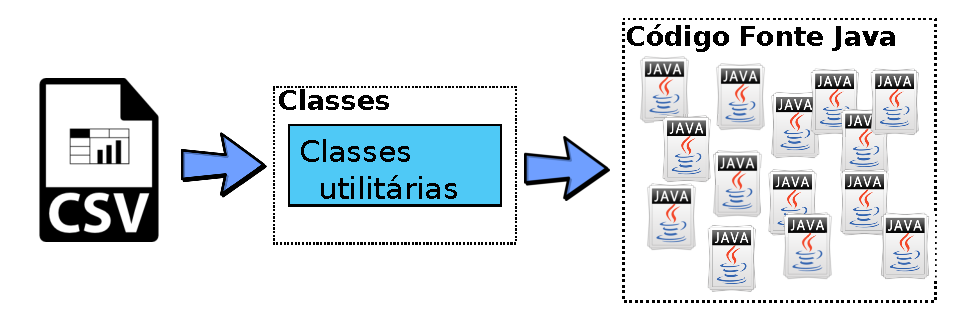
\includegraphics[scale=0.53]{Imagens/InputArquitetura}
%% 	\label{fig:InputArquitetura}
%% 	\caption{Input analisador estático.}
%% \end{figure}


\subsection{Análise da Representação Intermediária}

Conforme mencionado na Seção anterior \ref{sec:funcionamento}, o resultado da representação intermediária de em um arquivo fonte é a instância da classe \texttt{CompilationUnit}, que corresponde a uma \acs{AST} com todas as definições de tipo e 
implementação de comportamento presentes em um módulo Java. A plataforma Eclipse JDT oferece uma infraestrutura 
de classes para realizar a travessia em uma \acs{AST}, usando o padrão de projeto \textit{visitor}. Dessa forma, 
foi feita uma implementação de biblioteca de \textit{visitors}, para extrair as informações presentes na representação intermediária.   

%% Após todos os código fontes Java identificado é dado início a verificação destes arquivos onde são processados e gerado um \textit{parser} para que os \textit{visitors} pesquisam padrões previamente estabelecidos onde a pesquisa elaborada com o principal objetivo de reconhecer elementos e sua subestruturas contidos no código fonte.
%% Com isso a representação intermediária deste analisador é o processamento do código fonte para convertê-lo em um \textit{parser} para que os  \textit{visitor} realizem sua pesquisa. A Figura~\ref{fig:FuncionamentoAnalisador} demonstra o mais alto nível do funcionamento deste projeto.

%% \begin{figure}[h]
%% 	\center
%% 	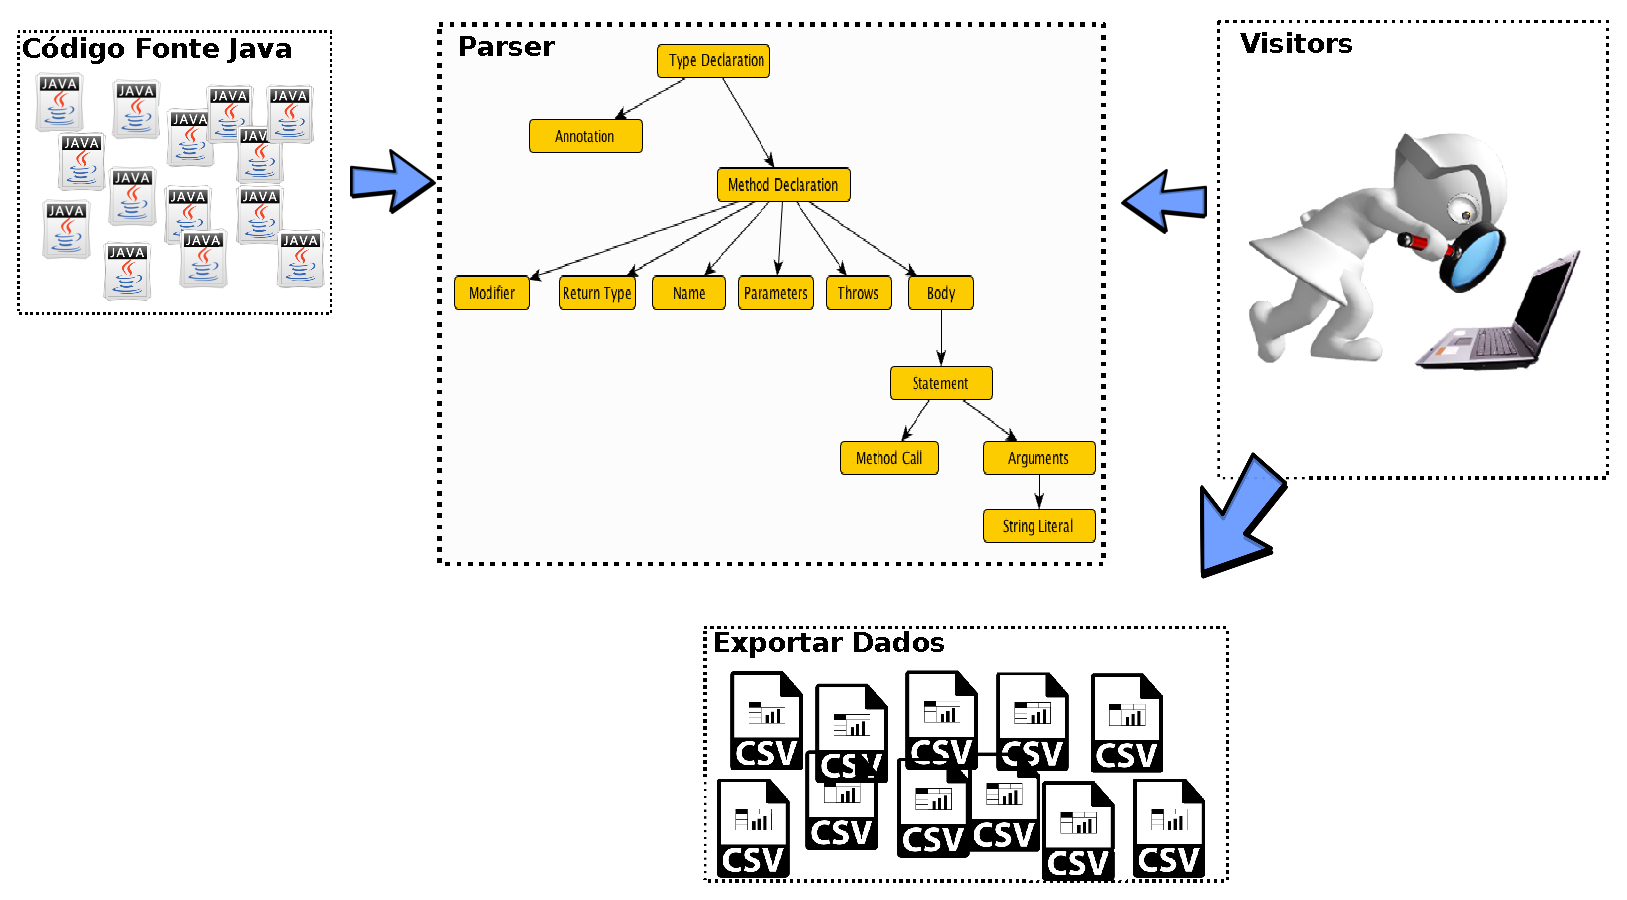
\includegraphics[scale=0.5]{Imagens/FuncionamentoVisitor}
%% 	\label{fig:FuncionamentoAnalisador}
%% 	\caption{Funcionamento analisador estático.}
%% \end{figure}

%{\color{red}{\bf rbonifacio}parece que ocorre uma transição muito abrupta de uma discussão alto nivel para uma discussão muito rica em detalhes.}

% De forma mais técnica, a representação intermediária, para cada arquivo fonte o analisador
% estático realiza a coleta de dados utilizando uma infraestrutura de \textit{visitors}. 

No contexto deste projeto, e objetivando um maior grau de reuso, toda classe \emph{visitor} precisa herdar de uma classe abstrata e parametrizada em relação a um tipo \texttt{T}, a classe \texttt{Visitor<T>}, onde o tipo \texttt{T} deve corresponder a classe usada para armazenar as informações coletadas pelo \emph{visitor}. O parâmetro de tipo \texttt{T} 
faz referência a uma classe composta basicamente por atributos e por operações de acesso (\textit{getters} e \textit{setters}), que serve para representar os dados extraídos. 

Em geral, de acordo com a arquitetura do analisador estático proposto, para cada construção que se deseja identificar o perfil de adoção nos projetos, são criadas duas classes: uma classe (\texttt{public class C\{ \ldots \}}) que representar as informações de interesse associadas ao uso de uma construção da linguagem Java e uma classe (\texttt{public class CVisitor extends Visitor<C> \{ \ldots \}}) que \emph{visita} a construção de interesse na árvore sintática abstrata. 

%Por exemplo, a Figura~\ref{fig:enum} apresenta o código necessário para visitar e popular informações relacionadas a declaração de enumerações. A classe \texttt{public class Visitor<T> \{ \ldots \}} possui uma coleção de objetos do tipo parametrizado, sendo possível adicionar instâncias desses objetos com a chamada \texttt{collectedData.addValue()}. Note que o exemplo apresentado corresponde a um dos mais simples \emph{visitors} implementados. Outros \emph{visitors} possuem uma lógica mais elaborada, como por exemplo os \emph{visitors} que identificam oportunidades para usar construções 
%como \emph{multi-catch} ou \emph{lambda expressions}. 

%\begin{figure}[ht!]
%\begin{lstlisting}
%public class EnumDeclaration {
%  private String file;
%  private int startLine;
%  private int endLine;
%	
%  //constructor + getters and setters.
%}
%
%public class EnumDeclarationVisitor extends Visitor<EnumDeclaration> {
%
%  @Override
%  public boolean visit(org.eclipse.jdt.core.dom.EnumDeclaration node) {
%    
%    EnumDeclaration dec = new EnumDeclaration(...);
%		
%    collectedData.addValue(dec);
%
%    return true;
%  }
%
%}
%\end{lstlisting}
%\label{fig:enum}
%\caption{Classes usadas para capturar declarações de enumerações.}
%\end{figure}


%% O diagrama da Figura~\ref*{fig:DiagramaVisitor} 
%% exibe de maneira técnica o procedimento de criar um \textit{Visitor} que detecte e colete informações dos tipos declarados no sistema, basta criar uma classes modelo \textit{TypeDeclaration.java} e  setar o parâmetro \textbf{<T>} como \textit{<TypeDeclaration>}, com isso os dados serão extraídas pelo \textit{Visitor, TypeDeclarationVisitor.java}, que identifica as informações pertinentes. {\color{red}refletir se esse parágrafo eh necessário}

%% \begin{figure}[h]
%% 	\center
%% 	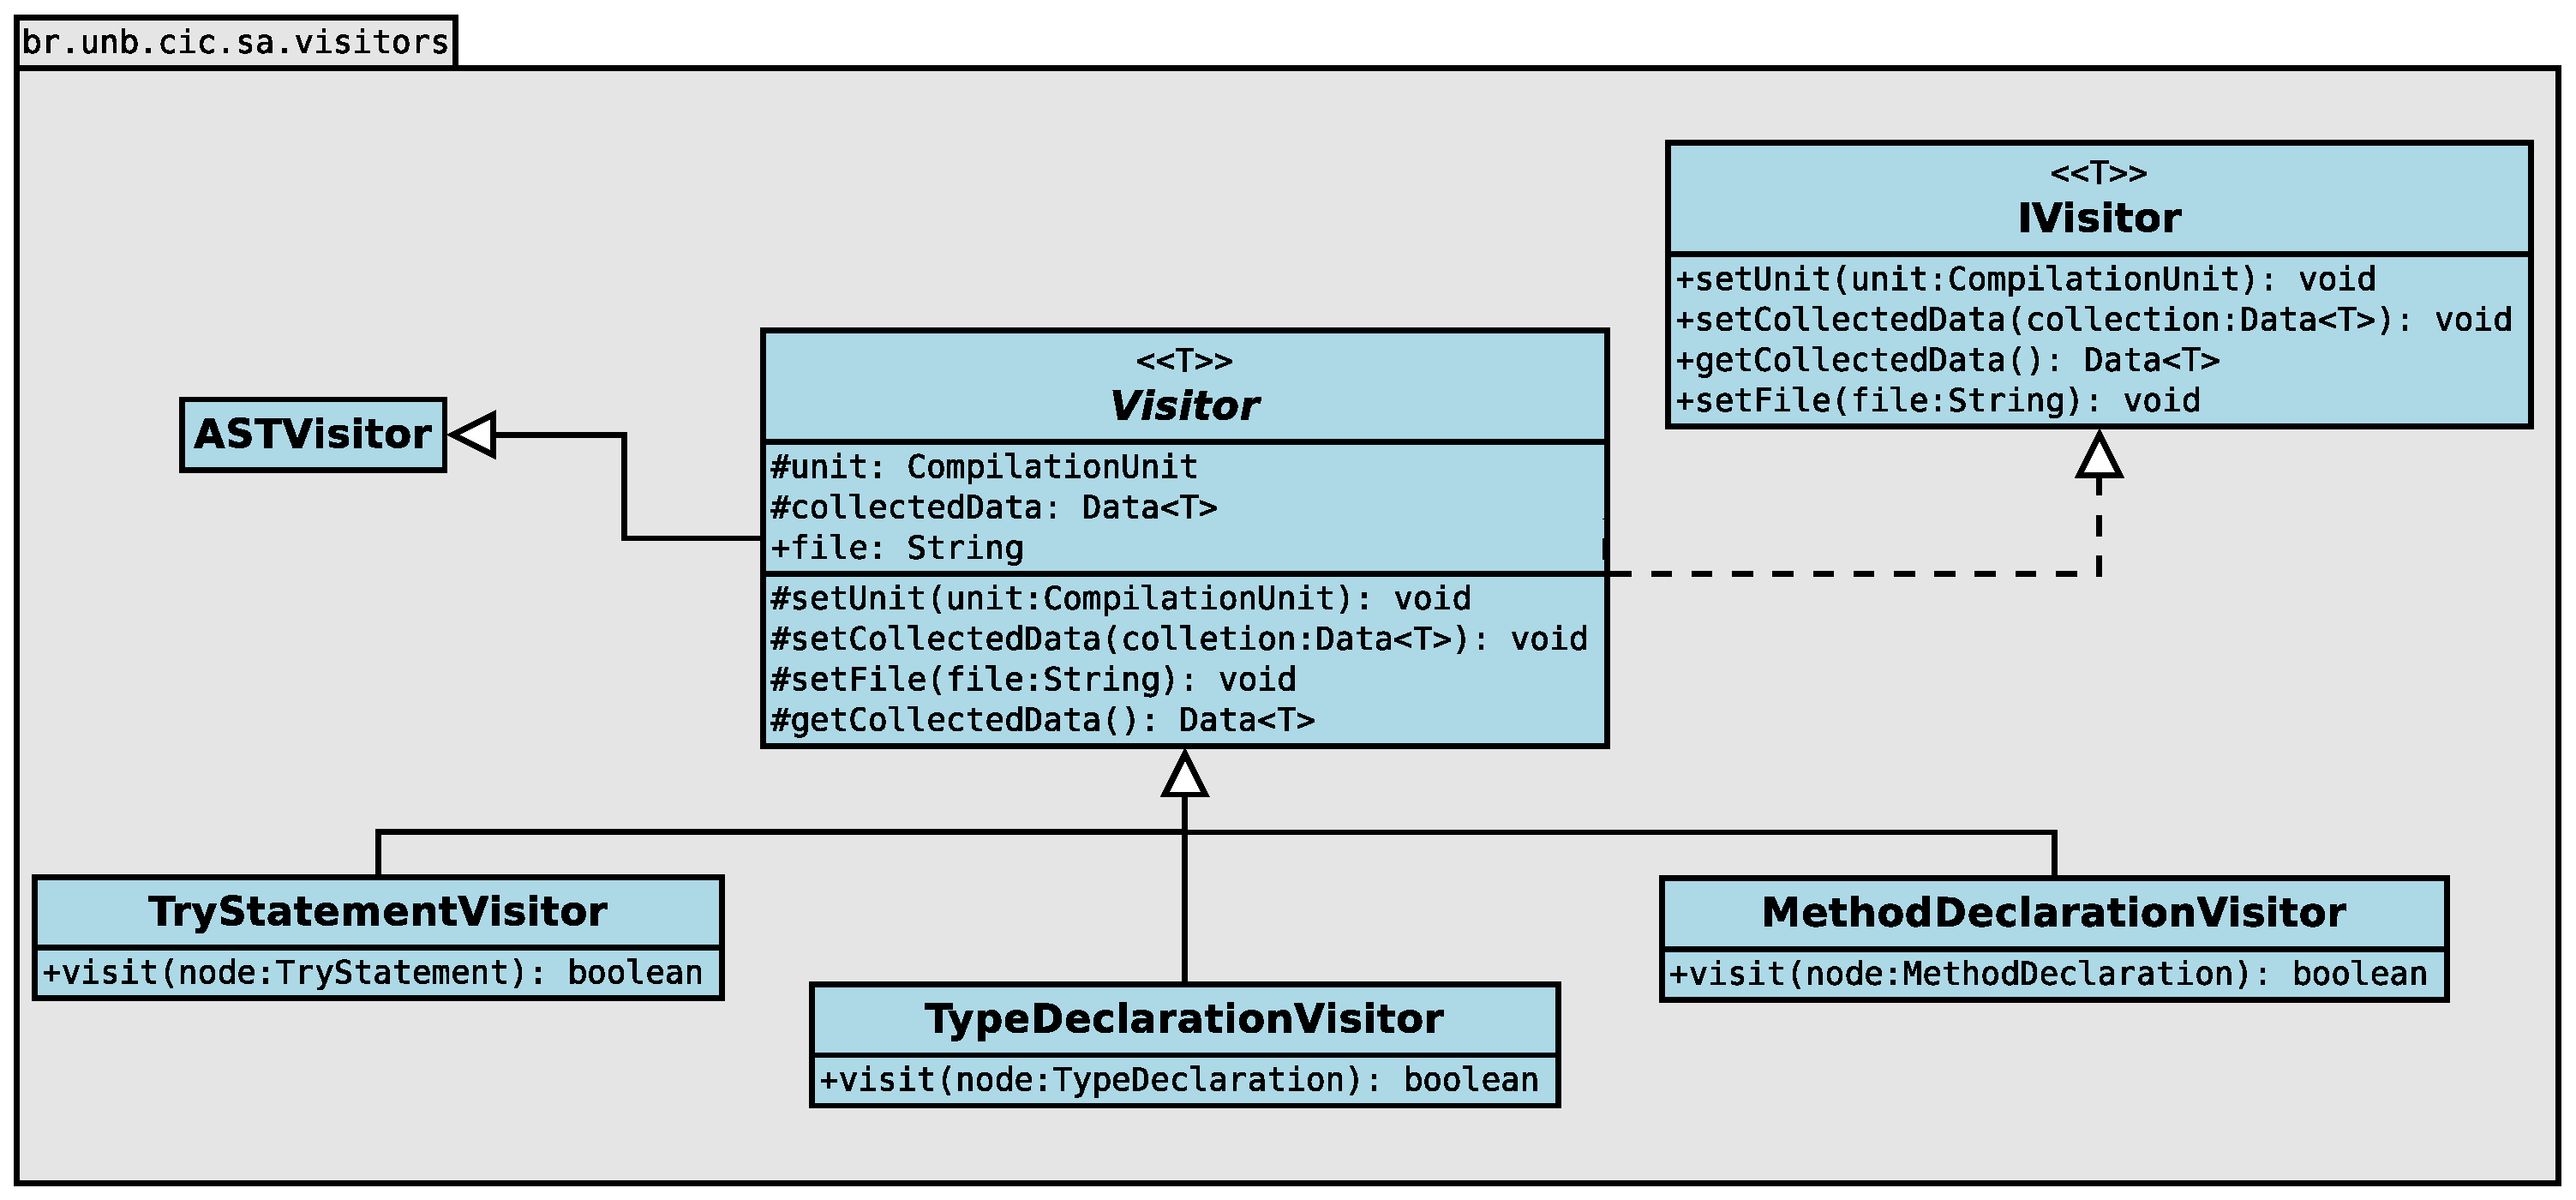
\includegraphics[scale=0.25]{Imagens/diagramaVisitor}
%% 	\label{fig:DiagramaVisitor}
%% 	\caption{Funcionamento analisador estático.}
%% \end{figure}

\subsubsection{Descrição dos Visitors}
Os \textit{visitors} implementados neste projeto 
são brevemente descritos a seguir, enquanto que 
a Tabela~\ref{tab:VisitorsCriados} apresenta 
duas métricas relacionadas à complexidade 
de implementação, em termos de 
complexidade ciclomática e total de linhas de código fonte. 
A complexidade ciclomática é dada pela quantidade de caminhos independentes 
em um trecho de código, enquanto que a quantidade de linhas de código 
foi computada ignorando comentários e linhas em branco.  Vale 
ressaltar que a complexidade ciclomática 
dos \textit{visitors} varia entre um e oito  (com a média igual a 2.5). A 
quantidade média de linhas de código necessária para escrever um 
\textit{visitor} é 47.

\begin{itemize}
\item \texttt{AIC:} Coleta informações relacionadas a declaração de 
\textit{Anonymous Inner Classes}. Tal informação é útil 
para estimar oportunidades de uso de expressões lambda. 

\item \texttt{ExistPattern:} Coleta informações de laços \texttt{foreach} 
que iteram sobre uma coleção com o intuito de verificar se um 
determinado objeto está presente na coleção. Tal informação é útil 
para estimar oportunidades de uso de expressões lambda. 


\item \texttt{FieldAndVariableDeclaration:} Coleta informações relacionadas 
a declarações de atributos e variáveis, com o intuito de 
extrair informações sobre a adoção de Java Generics. 

\item \texttt{FilterPattern:} Coleta informações de laços \texttt{foreach} 
que iteram sobre uma coleção com o intuito de 
filtrar elementos presentes na coleção. Tal informação é útil
para estimar oportunidades de uso de expressões lambda. 

\item \texttt{ImportDeclaration:} Coleta informações relacionadas à
importação de bibliotecas, sendo útil para estimar a adoção 
de bibliotecas voltadas para programação concorrente ou integração 
com linguagens de \textit{scripting}, por exemplo. 

\item \texttt{LambdaExpression:} Coleta informações relacionadas à 
adoção de expressões lambda. 

\item \texttt{Lock:} Verifica se os métodos utilizam algum dos mecanismos 
de \emph{lock} suportados diretamente pela linguagem Java, como \texttt{Lock}, 
\texttt{ReentrantLock}, \texttt{ReadLock} ou \texttt{WriteLock}.

\item \texttt{MapPattern:} Coleta informações de laços \texttt{foreach} 
que iteram sobre uma coleção com o intuito de 
aplicar alguma operação sobre os elementos presentes na coleção. 
Tal informação é útil 
para estimar oportunidades de uso de expressões lambda. 

\item \texttt{MethodCall:} Coleta informações relacionadas às 
chamadas de método, sendo \'{u}til para estimar o uso da API de 
introspecção de código, por exemplo. 

\item \texttt{MethodDeclaration:} Coleta informações relacionadas 
às declarações de métodos, sendo útil para identificar 
padrões de uso de Java Generics, por exemplo.

\item \texttt{ScriptEngine:} Coleta informações relacionadas 
ao uso da API Java para integração com linguagens de \textit{scripting}.  

\item \texttt{SwitchStatement:} Coleta informações relacionadas 
ao uso de sentenças \texttt{switch-case}, com o intuito principal 
de identificar o uso de \texttt{strings} nesse tipo de sentença. 

\item \texttt{SwitchString:} Coleta informações associadas às 
oportunidades de reestruturação de código para usar 
sentenças \texttt{switch-case} com \texttt{strings}. 

\item \texttt{TryStatement:} Coleta informações relacionadas 
ao uso de blocos \texttt{try-catch}, em particular para estimar o 
uso da construção \texttt{try-with-resources}. 

\item \texttt{TypeDeclaration:} Coleta informações sobre 
os tipos declarados (classes, interfaces, enumerações), com 
o intuito, por exemplo, de estimar a adoção de Java Generics. 
\end{itemize}

\begin{table}[ht] \footnotesize
	\centering
	\caption{Estimativa da complexidade de desenvolvimento de cada \emph{visitor}.}
	\label{tab:VisitorsCriados}	
    \begin{tabular}{crr}
%		\begin{tabular}{M|p{9cm}}% centered column
			\hline 
			Visitor &  \acs{CC} & \acs{LoC}\\ \hline \hline
			
			\texttt{AIC} & 6 & 64\\ 
			
			\texttt{ExistPattern}  & 28 & 116\\ 
			
			\texttt{FieldAndVariableDeclaration} & 8 & 81\\ 
			
			\texttt{FilterPattern}  & 43 & 168\\ 
			
			\texttt{ImportDeclaration}& 1 & 63\\ 
			
			\texttt{LambdaExpression} & 1 & 33\\ 
			
			\texttt{Lock} & 12 & 75\\ 
			
			\texttt{MapPattern} & 27 & 103\\ 
			
			\texttt{MethodCall} & 2 & 22\\ 
			
			\texttt{MethodDeclaration} & 5 & 45\\ 
			
			\texttt{ScriptingEngine} & 5 & 39\\ 
			
			\texttt{SwitchStatement} & 3 & 35\\ 
			
			\texttt{SwitchStringOpportunities} & 3 & 50\\ 
		
			\texttt{TryStatement} & 11 & 80\\ 
			
			\texttt{TypeDeclaration} & 2 & 41\\ \hline
		\end{tabular}
\end{table}

% \section{Exportação dos dados}

%% Para exportar os dados coletadas, foi construída uma solução extensível, baseada no padrão 
%% \emph{Injeção de Dependência} e introspecção de código. 
%% %\subsection{Injeçao de Dependência}


%\subsubsection{Extensibilidade para Inclusão de Novos Visitors}

%Para tornar a solução mais extensível, foram utilizados os mecanismos de 
%\emph{Injeção de Dependência} e introspecção de código. 
%Injeção de dependência (\emph{Dependency Injection}, \acs{DI}), 
%é um mecanismo de extensibilidade mais 
%conhecido como um padrão de projeto originalmente denominado de inversão de controle (\emph{Inversion of Control}, \acs{IoC}). 
%De acordo com esse mecanismo, a sequência de criação dos objetos depende de como os mesmos são 
%solicitados pelo sistema. Ou seja, quando um sistema é iniciado, 
%os objetos necessários são instanciados e injetados de forma apropriada, 
%geralmente de acordo com arquivo de configurações.
%O mecanismo de injeção de dependência foi incorporado na arquitetura 
%com o uso do \textit{framework} Spring~\cite{SPRING_REF}, o que não causou 
%nenhum impacto significativo na solução inicialmente proposta e que não 
%fazia uso de tal mecanismo--- nesse caso, os \emph{visitors} eram instanciados de maneira 
%\emph{programática}. O uso do mecanismo de injeção de dependência 
%serviu para flexibilizar não apenas a incorporação de novos \emph{visitors}, 
%mas também para definir, de forma mais flexível, a estratégia de exportação dos dados 
%coletados. Graças ao mecanismo de injeção de dependência, o desenvolvedor pode 
%concentrar seu esforço na criação de \textit{visitors}, fazendo como que estes implementem a 
%lógica necessária para extrair as informações. Para que novos \emph{visitors} se conectem 
%à plataforma, tornou-se necessário declarar o \textit{visitor} no arquivo com a definição 
%dos objetos gerenciados pelo Spring~\cite{SPRING_REF}.


\subsection{Exportação dos Dados}\label{subsec:exportacaoDados}

Na versão atual do suporte ferramental desenvolvido nessa monografia, os dados 
coletados pelo analisador estático são exportados exclusivamente no formato 
\acs{CSV}. Esse formato facilita as análises estatísticas usando o ambiente e linguagem 
de programação R~\cite{R}. Também com foco na extensibilidade do sistema, os componentes envolvidos na 
geração de relatórios utilizam os mecanismos de injeção de dependência, mencionado na 
seção anterior, e introspecção de código, via \acs{API} \textit{Reflection} da linguagem de 
programação Java. Tal mecanismo oferece aos programadores a capacidade de escrever componentes 
que podem observar e até modificar a estrutura e o comportamento dos objetos em tempo de execução.

A geração dos relatórios utiliza a classe \texttt{public class CSVData<T> \{ \ldots \ \}} onde o 
tipo parametrizado \texttt{<T>} é o mesmo utilizado para representar 
os dados coletados pelos \textit{visitors}. 
Os dados são obtidos através dos métodos de acesso (\textit{getters}) destas 
classes e exportados para arquivos~\acs{CSV}. 
O método \textit{export()} da classe \textbf{CSVData<T>} descobre quais dados são armazenados nos objetos do 
tipo \textbf{<T>}, usando o mecanismo de introspecção de código. Com isso, é possível 
generalizar a implementação e simplificar a exportação de dados coletados a partir de 
\textit{visitors} específicos. Ou seja, após a descoberta dos dados coletados pelos \textit{visitors} usando 
introspecção, é possível recuperar os mesmos assumindo a existência de métodos de 
acesso (\textit{getters} de acordo com a especificação Java Beans) e, 
como isso, exportá-los em arquivos \acs{CSV} de saída. 
A Figura~\ref{fig:exportacao} apresenta o uso desse mecanismo para generalizar a exportação dos 
dados. 

\begin{figure}[ht!]
\begin{lstlisting}[language=Java]
public class CSVData<T> implements Data<T> {

  @Override
  public void export() {
    StringBuffer str = new StringBuffer("");
      
    if(data == null) { return; }
      
    for(T value : data) {
      //reflection code...
      for(Field f: value.getClass().getDeclaredFields()){
	  
	String fieldName = f.getName();
	String prefix = "get";
	  
	if(f.getType().isPrimitive() && f.getType().equals(Boolean.TYPE)) {
	  prefix = "is";
	}
					
	String methodName = prefix +
	Character.toUpperCase(fieldName.charAt(0)) +
	fieldName.substring(1);
	  
	Method m = value.getClass().getDeclaredMethod(methodName);						
	str.append(m.invoke(value));
	str.append(";");
	
	writer.append(str.toString());
	writer.append("\n");			
		
	writer.flush();  
      }
    }
  }
\end{lstlisting}
\label{fig:exportacao}
\caption{Exportação de dados usando o mecanismo de introspecção de código.}
\end{figure}

%Projetar um analisador estático para extrair informações de softwares desenvolvido não é uma simples tarefa, entretanto EclipseJDT~\cite{EclipseJDT} prove uma abstração significativa tornado menos árdua este projeto. O que pode possibilitar projetar uma arquitetura mais robusta para este analisador onde o foco de qualquer desenvolvedor que deseje utilizá-lo concentre-se apenas na produção de seus \textit{Visitors}. 
%
%Um ponto de extrema relevância foi tornar este analisador independente de qualquer plataforma e \acs{IDE} foi um ponto vital para o concepção deste projeto que não tem como intuito ser plugin de qualquer \acs{IDE} o que acarretaria na limitação do seu uso a um cenário específico mas sim uma ferramenta para apoiar no desenvolvimento de um software com construções atuais. Utilizando a portabilidade nativa entre as plataformas provido pela linguagem Java este trabalho foi concebido com intuito de atender ao mais diversos desenvolvedores quer utilizem Linux, Windows, Mac ou qualquer outro sistema operacional que tenha suporte para Java.
%
%A análise tem como início a seleção de projetos, nesse caso seleção em repositórios públicos, onde após o download é informado analisador o diretório raiz onde estes estão localizados. Após é iniciado uma listagem dos arquivos fonte Java contidos nos projeto e contabilizados o total de \acs{LOC} e criado uma árvore sintática para cada arquivo encontrado através de um \textit{parser} provido pela biblioteca EclipseJDT~\cite{EclipseJDT}. Em seguida os \textit{Visitors} são instanciados com o objetivo de percorrer os nós destas árvores para pesquisar por construções de código previamente determinadas.
%
%Todas as construções pesquisadas quando encontradas pelos \textit{Visitors} são armazenadas temporariamente enquanto o analisador verifica todo projeto, quando é verificado a última árvore sintática pelos \textit{Visitors} é iniciado o processo de exportar os dados encontrados para um arquivo \acs{CSV} o conteúdo relevante destes blocos, a Figura~\ref{fig:Arquitetura} demostra de maneira clara o funcionamento do analisador. Após a exportação dos dados o analisador inicia todo processo novamente caso exista mais de um projeto.
%
%Devido ao mecanismo de \textit{reflection} proveniente da linguagem Java, o desenvolvedor não tem a necessidade de implementar código para exportação de dados tendo em vista que isto ocorre automaticamente através da introspecção realizada pelo analisador extraindo os dados armazenados pelos \textit{Visitors}.

%	\begin{figure}[h]
%		\center
%		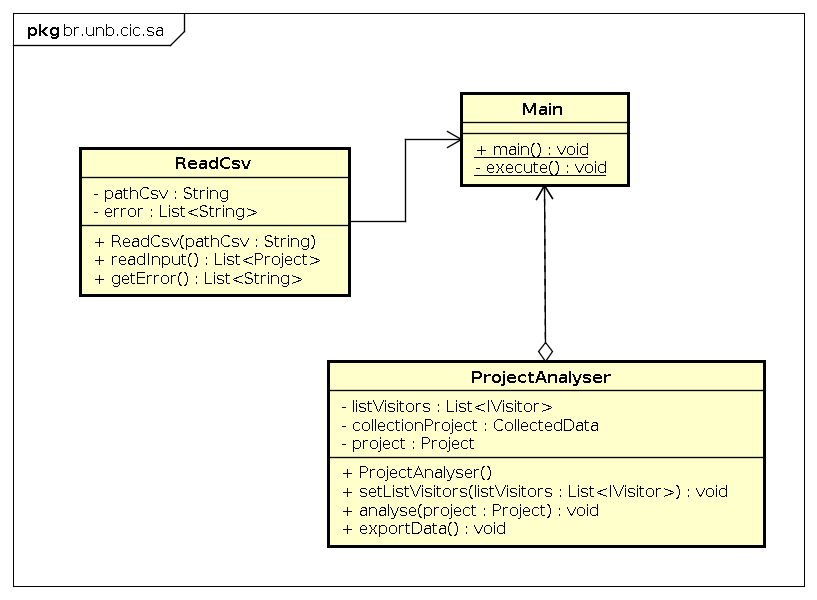
\includegraphics[scale=0.52]{Imagens/Arquitetura}
%		\label{fig:Arquitetura}
%		\caption{Funcionamento analisador estático.}
%	\end{figure}


%\section{Arquitetura}
%
%\subsection{Visitors}
%
%
%
%\begin{lstlisting}
%package br.unb.cic.sa.visitors;
%
%import org.eclipse.jdt.core.dom.ASTVisitor;
%import org.eclipse.jdt.core.dom.CompilationUnit;
%import br.unb.cic.sa.model.Data;
%
%public class Visitor<T> extends ASTVisitor implements IVisitor<T> {
%	protected CompilationUnit unit;
%	protected Data<T> collectedData;
%	protected String file;
%	
%	public Visitor() {}
%	
%	@Override
%	public void setUnit(CompilationUnit unit) { this.unit = unit; }
%	
%	@Override
%	public void setCollectedData(Data<T> colletion) { this.collectedData = colletion; }
%	
%	@Override
%	public void setFile(String file) {	this.file = file; }
%
%	@Override
%	public Data<T> getCollectedData() {	return collectedData;	}	
%}
%\end{lstlisting}
%
%
%A tabela:~\ref{tab:VisitorsCriados} detalha os 17 \textit{Visitors} criados com a respectiva descrição do trabalho realizado. Como forma de exemplificar a criação de um \textit{Visitors}, etapa a qual é composta de 4 passos quo serão demonstrados a seguir.
%
%A investigação para saber como o tratamento de exceção Java tem sido utilizado acarretou na criação de um \textit{Visitor} específico para este fim, \textit{TryStatementVisitor}, responsável por pesquisar este mecanismo o qual pode contar com alguma evoluções ao logo do histórico da linguagem Java. A pesquisa é iniciada encontrando blocos \textit{trys/catch}, onde destes será coletadas as informações referentes a adoção de \textit{resources} e oportunidade de utilizar \textit{multicatch} em blocos \textit{trys} que contenham \textit{catchs} iguais aninhados.
%%, neste caso de oportunidades os \textit{catchs} são testados por igualdade mas é trivial a utilização de um algoritmo mais avançado que teste a similaridade.
%
%Criação do \textit{Visitor TryStatementVisitor} com exemplo.
%
%	\begin{enumerate}
%		\item Inicialmente é necessário criar a classe modelo onde esta terá atribuição de receber os dados que serão extraídos pelos \textit{Visitors}, basicamente as classes modelos são compostas de \textit{getters} e \textit{setters} e são declaradas no pacote  \textit{\textbf{br.unb.cic.sa.model}}.
%			\begin{lstlisting}
%package br.unb.cic.sa.model;
%
%public class TryStatementData  {
%	private String file;
%	private int startLine;
%	private int endLine;
%	private boolean tryWithResource = false;
%	private boolean multiCatch = false;
%	
%	public TryStatementData(String file, int startLine, int endLine){
%		this.file = file;
%		this.startLine = startLine;
%		this.endLine = endLine;
%	}
%	
%	//getters and setters
%}
%			\end{lstlisting}
%			
%			
%		\item Em seguida, é concebida a criação do \textit{Visitor} no pacote \textit{\textbf{br.unb.cic.sa.visitors}} onde esta nova classe será estendida da classe parametrizada \textit{\textbf{Visitor<TryStatementData>}} apresentada anteriormente onde a parametrização desta classe é o modelo criado anteriormente.
%			
%			\begin{lstlisting}
%package br.unb.cic.sa.visitors;
%
%import java.util.List;
%import org.eclipse.jdt.core.dom.CatchClause;
%import org.eclipse.jdt.core.dom.TryStatement;
%import br.unb.cic.sa.model.TryStatementData;
%import br.unb.cic.sa.similarity.BasicSimilarityChecker;
%import br.unb.cic.sa.similarity.SimilarityChecker;
%
%public class TryStatementVisitor extends Visitor<TryStatementData> {
%
%	SimilarityChecker similarity;
%
%	public TryStatementVisitor() {
%		similarity = new BasicSimilarityChecker();
%	}
%
%	@Override
%	public boolean visit(s node) {
%
%		TryStatementData t = new TryStatementData(this.file, unit.getLineNumber(node.getStartPosition()),
%				unit.getLineNumber(node.getStartPosition() + node.getLength()));
%		
%		if (node.resources().size() > 0) {
%			t.setTryWithResource(true);
%		}
%	
%		if (node.catchClauses().size() > 1) {
%			if (this.checkSimilarity(node.catchClauses())) {
%				t.setMultiCatch(true);
%			}
%		}
%
%		this.collectedData.addValue(t);
%
%		return super.visit(node);
%	}
%	
%	private boolean checkSimilarity(List<CatchClause> catchClause) {
%		for (CatchClause cc : catchClause) {
%			for (CatchClause cn : catchClause) {
%				// To ignore the same catch in loops
%				if (!cc.equals(cn)) {
%				
%				//Chamada externa para testar similaridade
%					if (this.similarity.checkSimilarity(cc.getBody(),
%														cn.getBody())) {
%						return true;
%					}
%				}
%			}
%		}
%		return false;
%	}
%
%}
%			\end{lstlisting}
%			
%		 Na linha24, é testada a condição para saber se este bloco fez adoção de \textit{Resouce}. Na linha 30 é verificado que o bloco é um possível caso de \textit{multicatch} pois existe mais de um bloco. Na linha 39 tem-se o método \textit{checkSimilarity} o qual efetua a comparação dos blocos \textit{Catch} aninhados, entretando de forma trivial na linha 46, pode ser utilizado um algoritmo mais sofisticado para testar por similaridade modificando apenas o conteúdo do método \textbf{\textit{checkSimilarity}} da classe \textit{\textbf{SimilarityChecker}} o que não resulta em mudanças neste \textit{Visitor}.
%		
%	
%			\item Em seguida deve-se declarar o cabeçalho no arquivo \textit{resource/Beans.xml} do \textit{Spring} que estará presente no \acs{CSV} de saída. Onde este cabeçalho é composto pelo dados que serão extraídos pelos \textit{Visitors} e armazenados no modelo criado.
%			
%			\begin{lstlisting}
%<bean id="tryStatementData" class="br.unb.cic.sa.model.CSVData">
%	<property name="outDir" value="output"/>
%	<property name="fileName" value="tryStatement"/>
%	<property name="head" value="typeProject, before, project, version, file, start, end, resource, multiCatch"/> 
%</bean>
%			\end{lstlisting}
%			
%			
%			\item Por fim declarar o \textit{Visitor} como um \textit{bean} do \textit{Spring} para que este seja injetado no projeto e assim realize sua pesquisa.
%			
%			\begin{lstlisting}
%<bean id="tryStatementVisitor" class="br.unb.cic.sa.visitors.TryStatementVisitor">
%	<property name="collectedData" ref="tryStatementData"/>
%</bean>
%			\end{lstlisting}
%			
%	\end{enumerate}
%
%
%
%\subsection{Exportar Dados}
%A exportação dos dados para \acs{CSV} é realizado de forma automática utilizando o mecanismo de \textit{reflection} fornecido por Java. A classe parametrizada \textbf{\textit{CSVData<T>}} no pacote \textbf{\textit{br.unb.cic.sa.model}} implementa a interface \textit{\textbf{Data<T>}} onde \textbf{\textit{<T>}} faz  aos modelos declarados para as informações coletadas.
%
%\begin{lstlisting}
%package br.unb.cic.sa.model;
%
%public interface Data<T> {
%	public void setProject(Project project);
%	public void addValue(T value);
%	public void export();
%	public int size();
%	public void clean();
%}
%\end{lstlisting}
%
%
%Onde o atributo \textit{String[] head} é injetado pelo \textit{Spring} pois fora declarado anteriormente na criação do visitor. O método \textbf\textit{{export()}}, na linha 23, é o método responsável para exportar os dados em seus respectivos \acs{CSV} pois este método recupera as informações contidas nas coleções populadas pelos \textit{Visitors} e com \textit{reflection} captura os campos declarados em especial para os métodos quais são pré-fixados com \textit{get ou is} que terão seus valores capturados para que sejam exportados.
%
%\begin{lstlisting}
%package br.unb.cic.sa.model;
%
%import java.io.File;
%import java.io.FileWriter;
%import java.io.IOException;
%import java.lang.reflect.Field;
%import java.lang.reflect.InvocationTargetException;
%import java.lang.reflect.Method;
%import java.util.ArrayList;
%import java.util.List;
%
%public class CSVData<T> implements Data<T>{
%
%	private Project project;
%	private String fileName;
%	private String outDir;
%	private String[] head; 
%	private List<T> data;
%
%	...
%	
%	@Override
%	public void export() {
%		
%		try (FileWriter writer = new FileWriter(this.makeCsv(head), true)){
%		
%			StringBuffer str = new StringBuffer("");
%
%			if(data == null) {
%				return;
%			}
%			
%			for(T value : data) {
%				str = new StringBuffer("");
%				
%				str.append(project.getTypeOfProject());
%				str.append(";");
%				str.append(project.getBefore());
%				str.append(";");
%				str.append(project.getProjectName());
%				str.append(";");
%				str.append(project.getProjectRevision());
%				str.append(";");
%			
%				for(Field f: value.getClass().getDeclaredFields()){
%										
%					String fieldName = f.getName();
%					String prefix = "get";
%					
%					if(f.getType().isPrimitive() &&
%					   f.getType().equals(Boolean.TYPE)) {
%						prefix = "is";
%					}
%					
%					String methodName = prefix + 
%								Character.toUpperCase(fieldName.charAt(0)) +
%								fieldName.substring(1);
%										
%					try {
%						Method m = value.getClass().getDeclaredMethod(methodName);						
%						str.append(m.invoke(value));
%						str.append(";");
%					}catch(
%							NoSuchMethodException | 
%							IllegalAccessException |
%							IllegalArgumentException |
%							InvocationTargetException e) {
%							
%						throw new RuntimeException("Type " + 
%											value.getClass().getName() +
%											" must have a method named " +
%											 methodName);
%					}
%				}
%				
%				writer.append(str.toString());
%				writer.append("\n");
%				
%			}
%		
%			writer.flush();
%		
%		}
%		catch(Exception e) {
%			e.printStackTrace();
%		}
%	}
%}
%
%\end{lstlisting}
